\section{Задача 1.33}
\subsection{Задание:}
Вычислить:
\\[1em]
$
	\begin{vmatrix}
		0 & 1 & 1 & 1 & \cdots & 1 & 1 \\
		1 & a_1 & 0 & 0 & \cdots & 0 & 0 \\
		1 & 0 & a_2 & 0 & \cdots & 0 & 0 \\
		\vdots & \vdots & \vdots & \vdots & \ddots & \vdots & \vdots \\
		1 & 0 & 0 & 0 & \cdots & a_{n-1} & 0 \\
		1 & 0 & 0 & 0 & \cdots & 0 & a_n \\
	\end{vmatrix}
$
\subsection{Решение:}
Можно заметить что для различных $ n $ определитель такой матрицы равен
$ |A| = -\sum \limits_{i=1}^n \dfrac{1}{a_i} \prod \limits_{i=1}^n a_i $
\\
Докажем методом математической индукции:
\\
При $ n = 2 $:
\\
$
	\begin{vmatrix}
		0 & 1 & 1 \\
		1 & a_1 & 0 \\
		1 & 0 & a_2 &
	\end{vmatrix}
	= -a_1 - a_2
$
\\
Если утверждение верно при $ n $, тогда при $ n + 1 $
\\
$
\begin{vmatrix}
	0 & 1 & 1 & 1 & \cdots & 1 & 1 \\
	1 & a_1 & 0 & 0 & \cdots & 0 & 0 \\
	1 & 0 & a_2 & 0 & \cdots & 0 & 0 \\
	\vdots & \vdots & \vdots & \vdots & \ddots & \vdots & \vdots \\
	1 & 0 & 0 & 0 & \cdots & a_{n} & 0 \\
	1 & 0 & 0 & 0 & \cdots & 0 & a_{n+1} \\
\end{vmatrix}
= (-1)^{n+2} \cdot (-1)^{n+1} \cdot
\begin{vmatrix}
	0 & 1 & 1 & 1 & \cdots & 1 & 1 \\
	1 & a_1 & 0 & 0 & \cdots & 0 & 0 \\
	1 & 0 & a_2 & 0 & \cdots & 0 & 0 \\
	\vdots & \vdots & \vdots & \vdots & \ddots & \vdots & \vdots \\
	1 & 0 & 0 & 0 & \cdots & a_{n-1} & 0 \\
	1 & 0 & 0 & 0 & \cdots & 0 & a_n \\
\end{vmatrix}
- \sum \limits_{i=1}^n \dfrac{1}{a_i} \prod \limits_{i=1}^{n+1} a_i =
- \sum \limits_{i=1}^{n+1} \dfrac{1}{a_i} \prod \limits_{i=1}^{n+1} a_i
$
\subsection{Выполним компьютерную проверку в среде Wolfram Mathematica:}
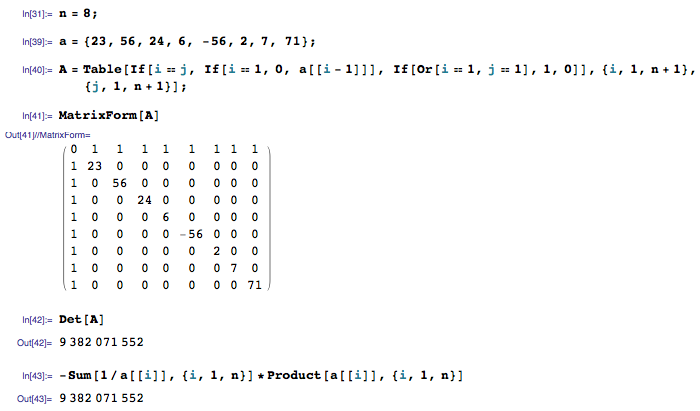
\includegraphics[scale=0.6]{task/1_33/screen.png}
\subsection{Вывод:}
Мы выполнили компьютерную проверку и убедились в верности предположения.
